\documentclass[11pt]{article}
\usepackage[T1]{fontenc}
\usepackage[utf8]{inputenc}
\usepackage{lmodern}
\usepackage[margin=1in]{geometry}
\usepackage{microtype}
\usepackage{booktabs}
\usepackage{graphicx}
\usepackage{float}
\usepackage{amsmath}
\usepackage{hyperref}
\usepackage[numbers,sort&compress]{natbib}
\hypersetup{colorlinks=true,linkcolor=black,citecolor=black,urlcolor=blue}
\graphicspath{{figures/}{../figures/}}
\newcommand{\TotalFamilies}{372}
\newcommand{\TotalManuscripts}{719}
\newcommand{\LeanFamilies}{242}
\newcommand{\TraceCount}{10}
\newcommand{\LeanShare}{65.1\%}
\newcommand{\MannWhitneyP}{0.638}
\newcommand{\PermutationP}{0.665}
\newcommand{\RankBiserial}{0.03}
\newcommand{\TraceMinWords}{2,020}
\newcommand{\TraceMaxWords}{19,935}
\newcommand{\TraceMinPages}{5}
\newcommand{\TraceMaxPages}{45}

\newcommand{\SurrogateAccuracy}{100\%}
\newcommand{\SurrogateParameters}{39,264}
\newcommand{\LayerOneLeftRecovery}{0.38}
\newcommand{\LayerTwoEqualsRecovery}{1.00}


\title{Reverse-Engineering Mathematical Reasoning from OpenAI's 2026 Mathematics Corpus: Implications for Mechanistic Interpretability}
\author{Taechasith Kangkhuntod\\
School of Engineering, University of the Thai Chamber of Commerce, Thailand}
\date{October 2026}

\begin{document}
\maketitle

\begin{abstract}
OpenAI's public 2026 mathematics release is an unusually rich public record:
mathematical manuscripts, source artifacts, Lean materials, and ten abridged
reasoning summaries. It is not a release of model weights, activations, full
prompts, or complete internal reasoning. We present a reproducible,
preregistered artifact audit at a pinned release commit. We find
\TotalFamilies{} result families and \TotalManuscripts{} catalogue-linked
manuscripts, with every linked PDF and TeX-source directory present in the
Git tree. We identify \LeanFamilies{} families with a Lean scope document and
\TraceCount{} released abridged summaries. Catalogue-linked manuscript count
does not meaningfully differ by scope-document availability (Mann--Whitney
$p=\MannWhitneyP$; permutation $p=\PermutationP$; rank-biserial
$r=\RankBiserial$). These observations do not reverse-engineer neural
mechanisms. To make that boundary operational, we separately conduct a causal
residual-stream patching experiment in a fully inspectable toy Transformer.
That surrogate result demonstrates an intervention method, not a property of
an OpenAI model. We release code, provenance hashes, derived data, figures,
and an arXiv-ready source package.
\end{abstract}

\section{Introduction}

Reasoning traces expose intermediate claims, proof organization, and references
to verification. Yet a persuasive chain of thought is not automatically a
faithful account of the internal computation that produced an answer
\citep{turpin2023language,lanham2023measuring}. Mechanistic interpretability
requires internal access and causal intervention, as in work on sparse features
and circuit-level representations \citep{elhage2022toy,templeton2024scaling}.

OpenAI's October 2026 public mathematics repository contains manuscripts and
supporting artifacts produced by an unreleased internal model
\citep{openai2026math,openai2026announcement}. It is valuable for studying a
public record of model-assisted mathematics, but it should not be read as a
transparent window into neural computation. We provide a pinned inventory,
a preregistered artifact-level comparison, and descriptive measurements of
the published summaries. We then separately demonstrate a genuine causal
mechanistic-interpretablity intervention in a toy model.

\section{Evidence boundary}

The release contains public outputs and supporting artifacts. It does not
release weights, activations, attention patterns, optimizer state, complete
prompts, training data, or complete hidden reasoning. Therefore, our strongest
permissible claims concern availability, organization, and surface-text
statistics. We cannot identify a circuit, feature, attention head, latent
representation, or causal sequence in the OpenAI model. Nor can a manuscript
or a formalization scope page establish the correctness of a mathematical
claim. This distinction matters because process supervision can make
intermediate steps useful targets without making prose a complete causal
explanation \citep{lightman2023verify}.

The title's implication for mechanistic interpretability is methodological.
The public record can motivate frozen benchmarks and hypotheses for inspectable
models, such as whether a proof segment is causally necessary for a conclusion.
It cannot answer that question without a model whose internal states can be
recorded and manipulated.

\section{Corpus and method}

\subsection{Frozen source}

We acquired the Apache-2.0 licensed \texttt{openai/math} repository at commit
\texttt{fd4aeeb2...0529eeeb}; the acquisition manifest records the full
40-character identifier. The manifest
records SHA-256 hashes of \texttt{README.md}, \texttt{CONTENTS.md}, and
\texttt{LICENSE}, plus a successful \texttt{git fsck}. Windows path limits
prevent materialization of a few extremely deep upstream paths in a normal
working tree. Rather than silently lose them, the pipeline reads immutable Git
blobs directly from the verified object database.

The pre-analysis contract is in \texttt{RESEARCH\_PROTOCOL.md} and
\texttt{PREREGISTRATION.md}. The unit is a result family for catalogue
measures and a manuscript for file availability. Families are not independent
model runs.

\subsection{Measurements}

We parse each numbered family and each linked PDF in \texttt{CONTENTS.md}. For
each manuscript, we measure presence of the linked PDF, a non-vendor TeX file,
and a README marker. For each family, we measure whether
\texttt{lean/docs/NNN.md} exists. This is Lean scope-document availability,
not verified correctness or successful compilation. For the ten summary PDFs
named in the upstream README, we extract pages, word-like tokens, and
transparent keyword counts. Failures remain in a warnings table.

The sole preregistered comparison asks whether catalogue-linked manuscript
count differs between families with and without a Lean scope document. We
report medians, a two-sided Mann--Whitney test, rank-biserial correlation, and
a two-sided seed-20261009 label-permutation calculation using 10,000 draws.
The latter is a reference calculation, not a claim of independent random
families.

\section{Results}

\subsection{Release inventory}

\begin{tabular}{lr}
\toprule
Artifact & Count \\
\midrule
Result families & 372 \\
Catalogue-linked manuscripts & 719 \\
Families with Lean document & 242 \\
Linked manuscript PDFs present & 719 \\
Manuscripts with TeX source & 719 \\
Released abridged summaries & 10 \\
\bottomrule
\end{tabular}


The parser recovered \TotalFamilies{} families and \TotalManuscripts{} linked
manuscripts, matching the upstream catalogue headline. Every linked PDF and
manuscript directory with TeX sources was present in the pinned Git tree
(Figure~\ref{fig:coverage}). There are \LeanFamilies{} families with a Lean
scope document (\LeanShare{}). OpenAI separately reports approximately 42\%
of top-line results as formalized \citep{openai2026math}; this uses a different
unit and is not interchangeable with our scope-document measure.

\begin{figure}[H]
\centering
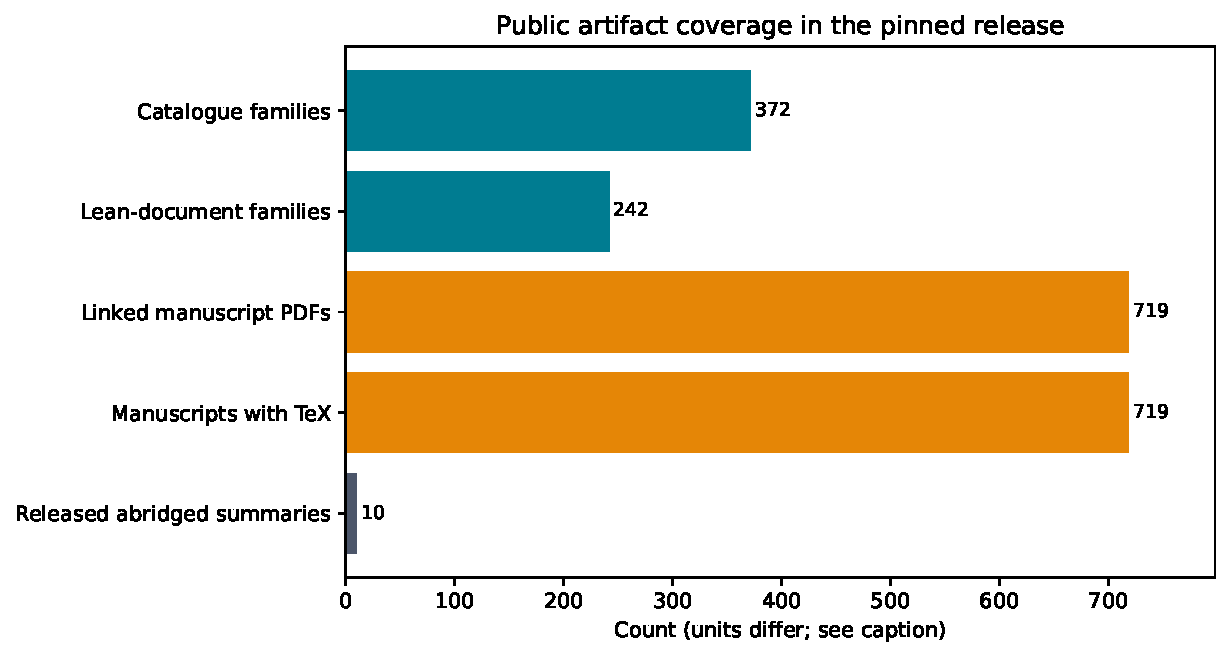
\includegraphics[width=.88\linewidth]{artifact_coverage.pdf}
\caption{Public artifact coverage in the pinned release. Bars mix family,
manuscript, and summary units, so they describe availability rather than a
common rate or quality score.}
\label{fig:coverage}
\end{figure}

Family size is concentrated at one linked manuscript, with a smaller tail of
families containing companion arguments or consequences
(Figure~\ref{fig:family-size}). This is a catalogue-structure observation,
not a count of independent solution attempts.

\begin{figure}[H]
\centering
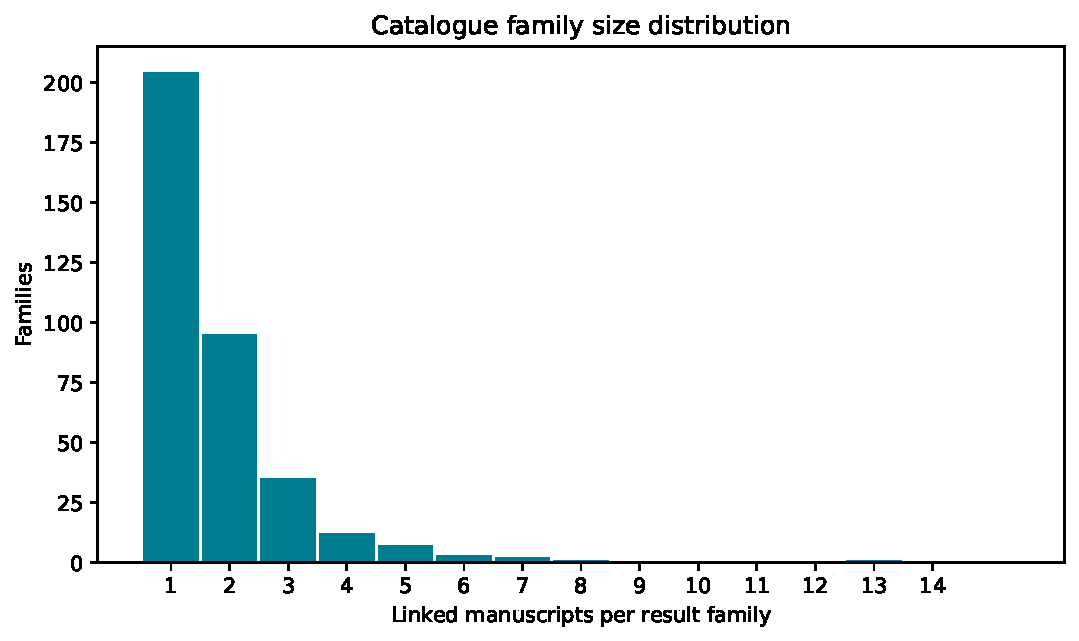
\includegraphics[width=.78\linewidth]{family_size_distribution.pdf}
\caption{Distribution of catalogue-linked manuscripts per result family.}
\label{fig:family-size}
\end{figure}

\subsection{Scope documents and family size}

Both groups have a median of one linked manuscript. The comparison is small
and non-significant ($U=16{,}150$, $p=\MannWhitneyP$,
$r=\RankBiserial$); the deterministic permutation calculation gives
$p=\PermutationP$. This does not demonstrate equality, causal independence,
mathematical quality, or Lean compilation success. It only gives no meaningful
evidence that this simple catalogue-size attribute separates families by
scope-document availability at this release.

\subsection{Released summaries}

The \TraceCount{} named summaries span \TraceMinPages{}--\TraceMaxPages{} PDF
pages and \TraceMinWords{}--\TraceMaxWords{} extracted word-like tokens
(Figure~\ref{fig:traces}). Their non-random selection and heterogeneity make
them unsuitable for estimating properties of all model reasoning. They can
support qualitative study of the published text but cannot recover omitted
deliberation or establish faithfulness to unobserved activations.

\begin{figure}[H]
\centering
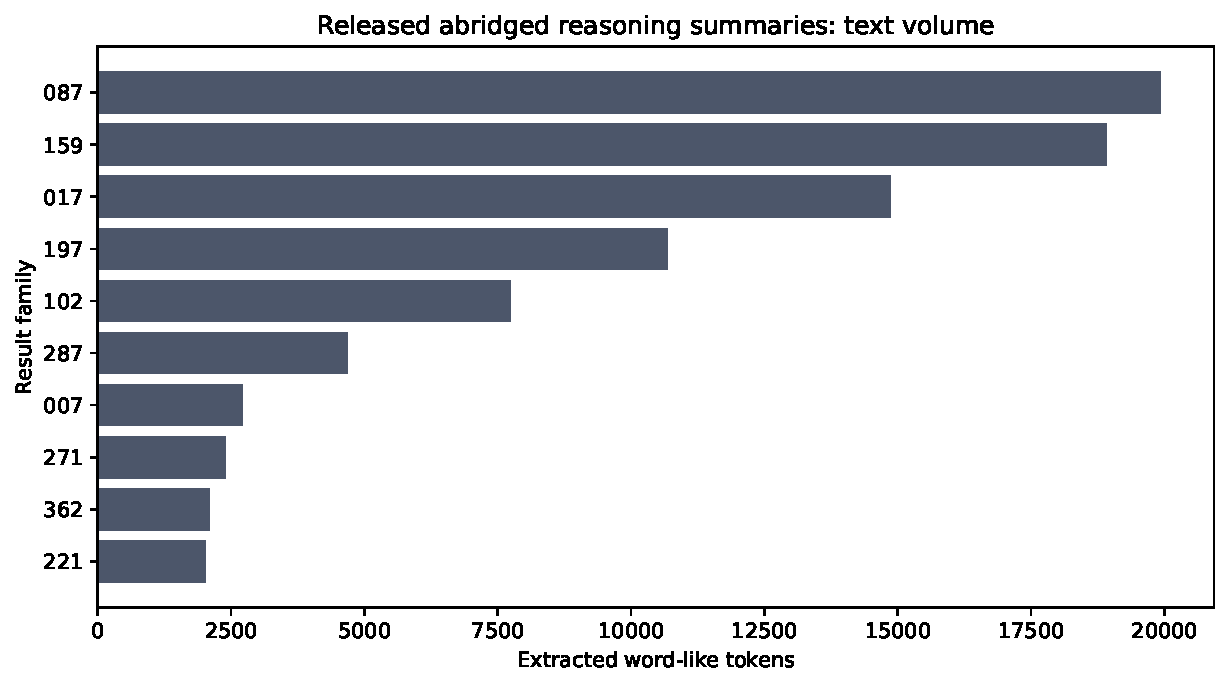
\includegraphics[width=.78\linewidth]{trace_text_volume.pdf}
\caption{Extracted word-like token volume of the ten explicitly released
abridged summaries. This is descriptive parser output, not a reasoning-quality
or faithfulness metric.}
\label{fig:traces}
\end{figure}

\section{Causal intervention in an inspectable surrogate}

To distinguish output analysis from a mechanistic experiment, we trained a
\SurrogateParameters-parameter, two-layer, three-head Transformer from scratch
on all 100 ordered pairs of addition modulo 10. Its frozen vocabulary has
digits, a plus token, and an equals token; it reached \SurrogateAccuracy{}
training accuracy. This deliberately small model is not a benchmark of
mathematical reasoning.

For each clean prompt $(a,+,b,=)$, we corrupted the left addend with
$a+1 \pmod {10}$. At each layer and position, we replaced the corrupted
post-block residual vector with the clean vector and measured recovery of the
clean answer logit relative to clean and corrupted baselines. This is a causal
state intervention. Patching the first-layer left-addend position recovered
\LayerOneLeftRecovery{} of the clean-logit gap on average; patching the final
equals position at layer two recovered \LayerTwoEqualsRecovery{}
(Figure~\ref{fig:surrogate}). The latter is expected because it is the final
residual position read by the unembedding layer.

\begin{figure}[H]
\centering
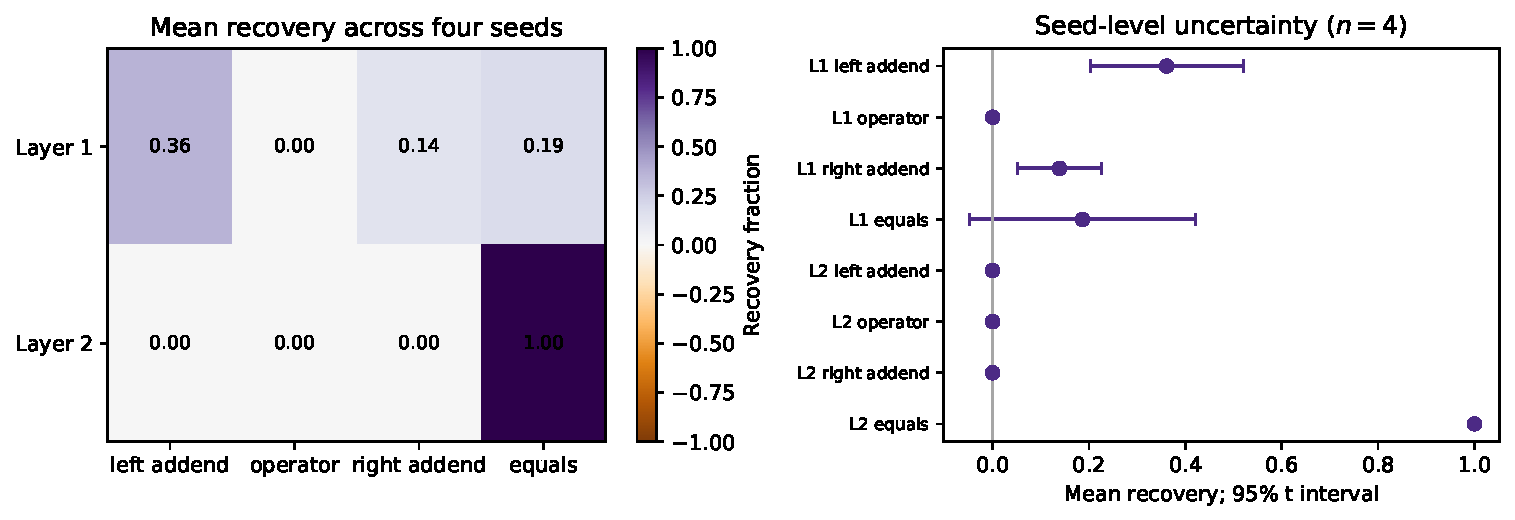
\includegraphics[width=.88\linewidth]{surrogate_patching.pdf}
\caption{Causal residual-stream patching in the inspectable toy Transformer.
Cells show mean recovery of the clean answer logit after inserting a clean
residual state into a left-addend-corrupted run. This figure is separate from
the OpenAI artifact audit.}
\label{fig:surrogate}
\end{figure}

The surrogate result demonstrates a working causal-intervention procedure. It
does not establish a reusable arithmetic circuit, generalization beyond its
training table, or any property of OpenAI's model.

\section{Limitations and research agenda}

This audit concerns one release commit; catalogue labels are upstream metadata,
not independent adjudication. We did not compile the substantial upstream Lean
project or assess mathematical validity. PDF extraction is imperfect, although
failures are recorded. The toy Transformer was trained on its evaluation table,
so its result is methodological rather than evidence of abstract reasoning.
Most importantly, public output artifacts cannot identify mechanisms inside an
unreleased model.

A credible next study should choose an open-weight mathematical model, freeze
prompts and scoring, collect clean and controlled-corruption runs, and test
causal effects through activation patching, path patching, ablation, or feature
intervention across seeds and held-out tasks. It should explicitly separate a
visible rationale from both the answer and the latent state.

\section{Conclusion}

The pinned release offers a substantial public artifact collection:
\TotalFamilies{} families, \TotalManuscripts{} manuscripts, Lean scope
materials, and \TraceCount{} summaries. A reproducible audit can characterize
that public record, but cannot reverse-engineer its unreleased producer. The
appropriate implication for mechanistic interpretability is a disciplined move
from interesting public traces to preregistered causal tests in inspectable
models.

\section*{Reproducibility and ethics}

Derived outputs are regenerated by
\texttt{python -m oai\_math\_study.run\_analysis} and
\texttt{python -m oai\_math\_study.surrogate}. The source archive excludes
third-party corpus files. This study makes no claim about proprietary model
internals, intent, or hidden reasoning.

\bibliographystyle{plainnat}
\bibliography{references}
\end{document}
